%%%%%%%%%%%%%%%%%%%%%%%%%%%%%%%%%%%%%%%%%%%%%%%%%%%%%%%%%%%%%%%%%%%%%
%% This is a (brief) model paper using the achemso class
%% The document class accepts keyval options, which should include
%% the target journal and optionally the manuscript type.
%%%%%%%%%%%%%%%%%%%%%%%%%%%%%%%%%%%%%%%%%%%%%%%%%%%%%%%%%%%%%%%%%%%%%
\documentclass[journal=jpclcd,manuscript=letter]{achemso}

%%%%%%%%%%%%%%%%%%%%%%%%%%%%%%%%%%%%%%%%%%%%%%%%%%%%%%%%%%%%%%%%%%%%%
%% Place any additional packages needed here.  Only include packages
%% which are essential, to avoid problems later. Do NOT use any
%% packages which require e-TeX (for example etoolbox): the e-TeX
%% extensions are not currently available on the ACS conversion
%% servers.
%%%%%%%%%%%%%%%%%%%%%%%%%%%%%%%%%%%%%%%%%%%%%%%%%%%%%%%%%%%%%%%%%%%%%
\usepackage[version=3]{mhchem} % Formula subscripts using \ce{}
\usepackage[T1]{fontenc}       % Use modern font encodings

\usepackage{color}
\usepackage{xr}
\externaldocument{master}

%%%%%%%%%%%%%%%%%%%%%%%%%%%%%%%%%%%%%%%%%%%%%%%%%%%%%%%%%%%%%%%%%%%%%
%% If issues arise when submitting your manuscript, you may want to
%% un-comment the next line.  This provides information on the
%% version of every file you have used.
%%%%%%%%%%%%%%%%%%%%%%%%%%%%%%%%%%%%%%%%%%%%%%%%%%%%%%%%%%%%%%%%%%%%%
%%\listfiles

%%%%%%%%%%%%%%%%%%%%%%%%%%%%%%%%%%%%%%%%%%%%%%%%%%%%%%%%%%%%%%%%%%%%%
%% Place any additional macros here.  Please use \newcommand* where
%% possible, and avoid layout-changing macros (which are not used
%% when typesetting).
%%%%%%%%%%%%%%%%%%%%%%%%%%%%%%%%%%%%%%%%%%%%%%%%%%%%%%%%%%%%%%%%%%%%%
\newcommand*\mycommand[1]{\texttt{\emph{#1}}}

\newcommand{\cli}{Cl$^{-}$}
\newcommand{\ki}{K$^{+}$}

\newcommand{\tsveta}[1]{\textcolor{red}{#1}}
\newcommand{\denis}[1]{\textcolor{green}{#1}}

%%%%%%%%%%%%%%%%%%%%%%%%%%%%%%%%%%%%%%%%%%%%%%%%%%%%%%%%%%%%%%%%%%%%%
%% Meta-data block
%% ---------------
%% Each author should be given as a separate \author command.
%%
%% Corresponding authors should have an e-mail given after the author
%% name as an \email command. Phone and fax numbers can be given
%% using \phone and \fax, respectively; this information is optional.
%%
%% The affiliation of authors is given after the authors; each
%% \affiliation command applies to all preceding authors not already
%% assigned an affiliation.
%%
%% The affiliation takes an option argument for the short name.  This
%% will typically be something like "University of Somewhere".
%%
%% The \altaffiliation macro should be used for new address, etc.
%% On the other hand, \alsoaffiliation is used on a per author basis
%% when authors are associated with multiple institutions.
%%%%%%%%%%%%%%%%%%%%%%%%%%%%%%%%%%%%%%%%%%%%%%%%%%%%%%%%%%%%%%%%%%%%%
\author{Tsveta Miteva}
\affiliation{Sorbonne Universit\'{e}, CNRS, Laboratoire de Chimie Physique Mati\`{e}re et Rayonnement, UMR 7614, F-75005 Paris, France}
\email{tsveta.miteva@upmc.fr}

\author{Nikolai V. Kryzhevoi}
\affiliation{Theoretische Chemie, Physikalisch-Chemisches Institut, Universit\"at Heidelberg, Im Neuenheimer Feld 229, D-69120 Heidelberg, Germany}

\author{Nicolas Sisourat}
\affiliation{Sorbonne Universit\'{e}, CNRS, Laboratoire de Chimie Physique Mati\`{e}re et Rayonnement, UMR 7614, F-75005 Paris, France}

\author{Christophe Nicolas}
\affiliation{Synchrotron SOLEIL, l`Orme des Merisiers, Saint-Aubin, F-91192 Gif-sur-Yvette Cedex, France}

\author{Wandared Pokapanich}
\affiliation{Faculty of Science, Nakhon Phanom University, Nakhon Phanom 48000, Thailand}
%
\author{Thanit Saisopa}
\author{Prayoon Songsiriritthigul}
\affiliation{School of Physics, Suranaree University of Technology, Nakhon Ratchasima 30000, Thailand}
%
\author{Yuttakarn Rattanachai}
\affiliation{Department of Applied Physics, Faculty of Sciences and Liberal Arts, Rajamangala University of Technology Isan, Nakhon Ratchasima 30000, Thailand}

\author{Andreas Dreuw}
\author{Jan Wenzel}
\affiliation{Interdisciplinary Center for Scientific Computing, Ruprecht-Karls University, Im Neuenheimer Feld 205A, D-69120 Heidelberg, Germany}

\author{J\'{e}r\^ome Palaudoux}
\affiliation{Sorbonne Universit\'{e}, CNRS, Laboratoire de Chimie Physique Mati\`{e}re et Rayonnement, UMR 7614, F-75005 Paris, France}

\author{Gunnar \"{O}hrwall}
\affiliation{MAX IV Laboratory, Lund University, P.O. Box 118, SE-22100 Lund, Sweden}

\author{Ralph P\"{u}ttner}
\affiliation{Fachbereich Physik, Freie Universit\"at Berlin, Arnimallee 14, D-14195, Berlin, Germany}

\author{Lorenz S. Cederbaum}
\affiliation{Theoretische Chemie, Physikalisch-Chemisches Institut, Universit\"at Heidelberg, Im Neuenheimer Feld 229, D-69120 Heidelberg, Germany}

\author{Jean-Pascal Rueff}
\affiliation{Sorbonne Universit\'{e}, CNRS, Laboratoire de Chimie Physique Mati\`{e}re et Rayonnement, UMR 7614, F-75005 Paris, France}
\alsoaffiliation{Synchrotron SOLEIL, l`Orme des Merisiers, Saint-Aubin, F-91192 Gif-sur-Yvette Cedex, France}

\author{Denis C\'{e}olin}
\email{denis.ceolin@synchrotron-soleil.fr}
\affiliation{Synchrotron SOLEIL, l`Orme des Merisiers, Saint-Aubin, F-91192 Gif-sur-Yvette Cedex, France}

%%%%%%%%%%%%%%%%%%%%%%%%%%%%%%%%%%%%%%%%%%%%%%%%%%%%%%%%%%%%%%%%%%%%%
%% The document title should be given as usual. Some journals require
%% a running title from the author: this should be supplied as an
%% optional argument to \title.
%%%%%%%%%%%%%%%%%%%%%%%%%%%%%%%%%%%%%%%%%%%%%%%%%%%%%%%%%%%%%%%%%%%%%
%<<<<<<< HEAD:suppinfo.tex
\title{The all-seeing eye of resonant Auger electron spectroscopy: a study on aqueous solution using tender x-rays}
%\title{Tracking the hazy boundary between resonant and normal Auger decay near the K-edges of aqueous \ki~and \cli}
%=======
\title{The all-seeing eye of resonant Auger electron spectroscopy: a study on aqueous KCl}
%\title{Tracking the hazy boundary between resonant and normal Auger decay in near the K-edges of aqueous \ki~and \cli}
%>>>>>>> origin/master:suppinfo - Copy.tex

%%%%%%%%%%%%%%%%%%%%%%%%%%%%%%%%%%%%%%%%%%%%%%%%%%%%%%%%%%%%%%%%%%%%%
%% Some journals require a list of abbreviations or keywords to be
%% supplied. These should be set up here, and will be printed after
%% the title and author information, if needed.
%%%%%%%%%%%%%%%%%%%%%%%%%%%%%%%%%%%%%%%%%%%%%%%%%%%%%%%%%%%%%%%%%%%%%
\abbreviations{AES,XAS}
\keywords{Solvated ions, Auger electron spectroscopy, x-ray absorption spectroscopy}
\renewcommand{\figurename}{Figure SI}
%%%%%%%%%%%%%%%%%%%%%%%%%%%%%%%%%%%%%%%%%%%%%%%%%%%%%%%%%%%%%%%%%%%%%
%% The manuscript does not need to include \maketitle, which is
%% executed automatically.
%%%%%%%%%%%%%%%%%%%%%%%%%%%%%%%%%%%%%%%%%%%%%%%%%%%%%%%%%%%%%%%%%%%%%
\begin{document}

\section{Methods}
\subsection{Experimental}

For the present experiment we used the newly operational microjet setup that was specifically designed for the HAXPES station of the GALAXIES beamline \citep{ceolin13:188,rueff15:175}. A differentially-pumped tube in which the microjet head is inserted, is mounted on a 3-axes motorized manipulator in front of the spectrometer lens. Two holes of 2\,mm diameter allow the photons to go in and out. At the end of the tube and in front of the lens, a 500\,$\mu$m diameter hole skimmer allows the electrons created at the interaction point to go in the direction of the spectrometer. The microjet head is mostly composed of a 30\,$\mu$m diameter vertical glass capillary facing a temperature-controlled catcher in CuBe having a 300\,$\mu$m hole, and a camera. Piezo motors allow their precise alignment relative to each other and to the photon beam. The catcher is placed at a distance of about 5\,mm from the capillary and is permanently pumped in order to extract the liquid. For the present experiment, a 0.5M KCl aqueous solution is injected in the capillary by a high performance liquid chromatography (HPLC) pump with a constant flux of 1.6\,ml/min. The alignment of the setup is performed on the KCl aqueous solution by measuring the water O1s x-ray photoelectron peak intensity and by optimizing the liquid vs gas phase ratio. The pressure in the main chamber is kept below the 10$^{-5}$\,mbar range whereas it is kept at about 10$^{-4}$\,mbar in the differentially-pumped tube when the HPLC pump is ON. Our equipment is an updated version of the equipment used in Ref.\ \cite{faubel88:269}. The aqueous potassium chloride solution was prepared by mixing >99\% KCl salt with deionized water. Filtering and degazing procedures were systematically performed before injecting the solution. The spectrometer resolution of about 0.6\,eV was achieved with the 500\,eV pass energy and 0.5\,mm slits. The photon energy resolution achieved at 2.8\,keV and 3.6\,keV was about 0.3\,eV and 0.4\,eV, respectively. The experimental 2D maps representing the evolution of the KLL Auger spectra in the vicinity of the Cl$^{-}$ and K$^{+}$~K-edges, as a function of the photon energy, are shown in Figs.\ \ref{fg:2dmap_k} and \ref{fg:2dmap_cl} in the main text, respectively. The aqueous K$^{+}$~and Cl$^{-}$~1s ionization potentials were measured at h$\nu = 5$\,keV and calibrated on the liquid contribution of the O1s XPS spectrum \cite{winter06:1176}. The maps were also calibrated using the O1s photoelectron line of liquid water but at photon energies close to the potassium and chloride 1s ionization thresholds.


\subsection{{\bf{\it Ab initio}} calculations}

The theoretical X-ray absorption spectra were computed for the hexa-coordinated clusters of both ions, K$^{+}$(H$_2$O)$_6$ and Cl$^{-}$(H$_2$O)$_6$, which can be considered as representatives of the complete first solvation shell of the two ions \citep{Ohtaki93:1157,soper06:180,ma14:1006}. The two structures shown in Fig.\ \ref{fg:xas_kcl} were optimized at the DFT level of theory using the B3LYP functional and the 6-311++G(2d,2p) basis set \citep{Krishnan80:650,Blaudeau97:5016}. The geometry optimization was performed with the Gaussian 09 package \citep{g09}. In order to obtain a realistic structure for K$^{+}$~corresponding to the bulk solution, we carried out constrained geometry optimization by choosing the equilibrium gas-phase geometries \citep{lee99:3995,lee02:5509} belonging to the D$_3$ point group and then increasing the angle $\theta$ between the K-O bond and the $C_3$ axis to 55$^{\circ}$. This angle was chosen such that the O-K-O angles are around the maxima of the angular distributions obtained from quantum mechanics/molecular mechanics simulations in Ref.\ \citep{ma14:1006}. Moreover, we fixed the K-O distance to 2.840~\AA, such that it corresponds to the distances from other theoretical and experimental works \citep{Ohtaki93:1157,soper06:180,ma14:1006}.


The energies and transition moments of the core excited states of the bare ions and microsolvated clusters were computed with the algebraic diagrammatic construction method for the polarization propagator \citep{sch82:2395} within the core-valence separation approximation \citep{bar85:867,ced80:206,ced81:1038} (CVS-ADC(2)x) as implemented in the Q-Chem package \citep{Wenzel14:1900,Wenzel14:4583,Wormit14:774,QChem2015}. In the case of Cl$^{-}$~the 6-311++G(3df,3pd) basis set \citep{Krishnan80:650,McLean80:5639} (excluding f functions) was used on all atoms, whereas in the case of K$^{+}$~we used the 6-311+G(2d,p) basis set \citep{Krishnan80:650,Blaudeau97:5016} on all atoms, and two additional sets of s, p and d diffuse functions were added on K. The use of a smaller basis set in the case of K is due to the higher number of atomic orbitals compared to the case of Cl, and therefore, prohibitively high cost of the CVS-ADC(2)x computation. In our calculations the core space comprises the 1s orbital of K$^{+}$ or Cl$^{-}$, whereas the remaining occupied orbitals are included in the valence space. For the calculations of the XAS spectra we used the C$_2$ point group in the case of K$^{+}$(H$_2$O)$_6$ and Cl$^{-}$(H$_2$O)$_6$. To account for the lifetime broadening due to the Auger decay of the core excited states, we convolved the theoretical spectra with a Lorentzian function of FWHM 0.74\,eV and 0.62\,eV in the case of K$^{+}$~and Cl$^{-}$, respectively \citep{Krause79:329}. Additionally, we convolved the theoretical spectra with a Gaussian profile to also account for the experimental resolution (see Fig.\ \ref{fg:xas_kcl} in the main text). We analyzed the core excited states by expanding the natural orbitals occupied by the excited electron (singly occupied natural orbitals, SONOs) $\psi_{i}$ of the microsolvated clusters in the basis of SONOs of the bare K$^{+}$ or Cl$^{-}$~ions, $\chi_{nl}$
%
\begin{equation}
\psi_{i} = \sum_{nl} a^{i}_{nl} \chi_{nl}
\end{equation}
%
where $n$ and $l$ stand for the principal and orbital quantum numbers as described in Ref.\ \citep{miteva16:16671}. The expansion coefficients $a^{i}_{nl}$ show the degree of delocalization of the excited electron and the mixing of the core excited states in the ligand field created by the surrounding water molecules (see Fig.\ \ref{fg:xas_kcl}).


The final states following KLL resonant Auger decay of K$^{+}$(H$_2$O)$_6$ and Cl$^{-}$(H$_2$O)$_6$ were computed at the Configuration Interaction Singles (CIS) level using the Graphical Unitary Group Approach (GUGA) as implemented in the GAMESS-US package \citep{GUGA_PhysScr_21,GUGA_JCP_70,GUS}. In order to account for the relaxation effects upon core ionization, we employed a restricted open-shell Hartree-Fock reference wave function with a hole in the 2s orbital of both K$^{+}$~and Cl$^{-}$.  We used the 6-311++G(2d,2p) basis set \citep{Krishnan80:650,McLean80:5639,Blaudeau97:5016} on all atoms. Additionally, the basis set was augmented with two sets of s, p, d diffuse functions in the case of K$^{+}$, and three sets of s, p, d diffuse functions in the case of Cl$^{-}$. The larger basis set employed in the case of Cl was necessary in order to ensure the convergence of the excited states. The active space comprises the 2s and 2p orbitals of K/Cl with occupancy fixed to 6 and all virtual orbitals with occupancy fixed to 1. The remaining doubly occupied orbitals were frozen in the calculation. \citep{mosnier16:061401}

\section{PCI shift}
In order to estimate the maximum amplitude of the PCI shift, we compare the positions of the normal KLL Auger lines of both Cl$^{-}_{\text{aq}}$ and K$^{+}_{\text{aq}}$ close to threshold with those recorded far from threshold, at photon energies h$\nu = 5$\,keV \citep{ceolin17:263003}. We observe a shift of $\sim$1\,eV of the maxima towards lower kinetic energies as compared to the spectra reported in \citep{ceolin17:263003}. The magnitude of the shift is constant in the photon energy range of $\sim$8\,eV above threshold and similar for the two ions. A possible explanation of the shift observed in our experiment is given in Ref.\ \cite{tchaplyguine07:124314} where it was proposed that it is due to a process of internal ionization, i.e.\ excitation of the photoelectron into the conduction band, followed by normal Auger decay. The observed shift was explained as resulting from the PCI-like interaction between the Auger electron and the electron excited to the conduction band.

\section{Core-excited states of Cl$^{-}$}
\begin{figure}[h!]
\centering
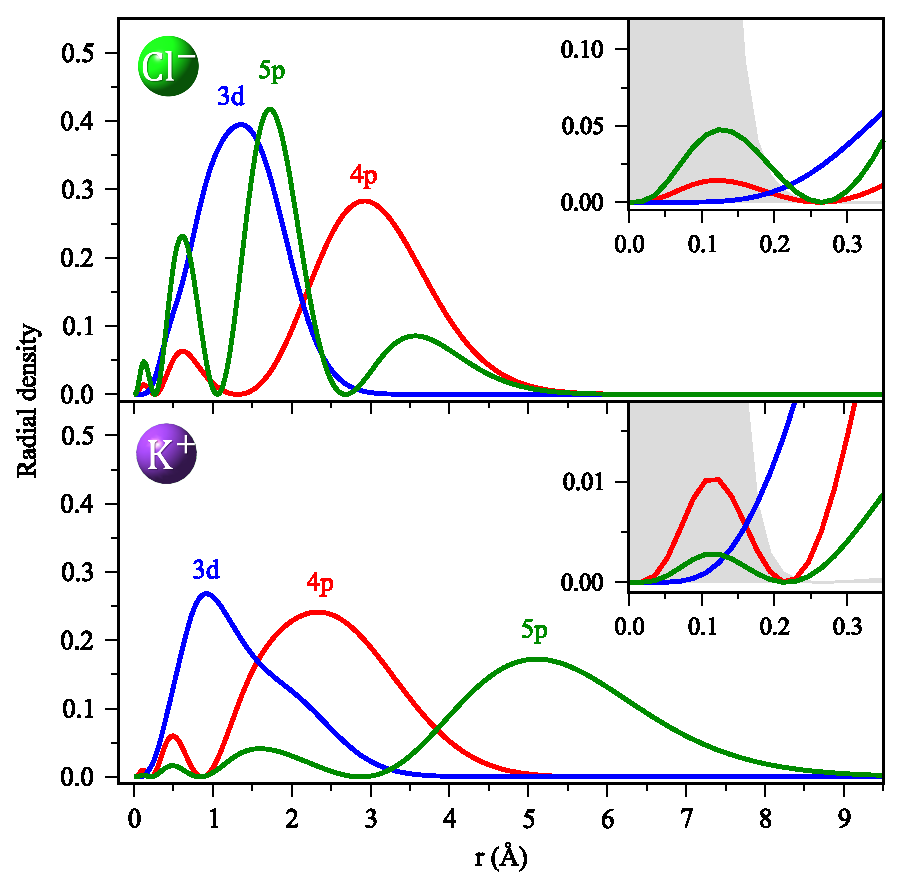
\includegraphics[scale=0.8]{figures/rad_dens_kcl.eps}
\caption{Radial density distributions of the singly-occupied natural orbital occupied by the excited electron corresponding to the 1s$^{-1}$4p, 1s$^{-1}$3d and 1s$^{-1}$5p core excitations in \ki~(lower panel) and \cli~(upper panel). The insets show the region of distances relevant for the overlap with the 1s core orbital whose radial density is shown as a grey shaded area.}
\label{fg:si_rdens_ions}
\end{figure}
%<<<<<<< HEAD:suppinfo.tex
%
%
The intensity of the Cl$^{-}$(1s$^{-1}$4p) state is lower than that of the \cli(1s$^{-1}$5p) state contrary to what is observed in \ki. This difference can be explained by the lower electron density of the 4p compared to the 5p electron in the region close to the core hole which thus results in the lower oscillator strength of the 1s$^{-1}$4p compared to the 1s$^{-1}$5p transition in \cli~(see Fig.\ \ref{fg:si_rdens_ions} in SI).
In what follows we give a simple explanation of the difference in the radial density distributions of the 1s$^{-1}$4p and 1s$^{-1}$5p states in \ki~and \cli. In the case of \ki, the excited electron mainly sees a $2/r$ potential. In addition, it sees a short range potential originating from the point-like nucleus and the screening electrons. The influence of the latter can be described by a quantum defect $\delta \ne 0$, which is almost constant for the entire infinite Rydberg series. However, in case of \cli~the outer electron does not experience a Coulomb potential and the short range potential becomes dominant. As a result of the absence of the Coulomb potential we see a different behavior in the properties of the states, like e.g.\ only a finite number of bound states (here obviously 4p) \citep{buckman94:539}. In contrast to this, the 3d and 5p states are not bound. % in the continuum.}
%=======

In what follows we give a simple explanation of the difference in the radial density distributions of the 1s$^{-1}$4p and 1s$^{-1}$5p states in \ki~and \cli. In the case of \ki, the excited electron mainly sees a $2/r$ potential. In addition, it sees a short range potential originating from the point-like nucleus and the screening electrons. The influence of the latter can be described by a quantum defect $\delta \ne 0$, which is almost constant for the entire infinite Rydberg series. However, in case of \cli~the outer electron does not experience a Coulomb potential and the short range potential becomes dominant. As a result of the absence of the Coulomb potential we see a different behavior in the properties of the states, like e.g.\ only a finite number of bound states (here obviously 4p) \citep{buckman94:539}. In contrast to this, the 3d and 5p states are not bound. % in the continuum.}


\begin{figure}
\centering
\includegraphics[scale=0.9]{figures/partial_cross_sec_ct_time.pdf}
\caption{Partial cross sections and charge transfer time extracted from Fig.\ \ref{fg:2dmap_cl}. The blue and red curves are obtained by integrating the area of the 2p$^{-2}$ and 2p$^{-2}$4p final states ($^1$D state region only) at each photon energy step. From these curves we determine the charge transfer time $\tau_{\text{CT}}$ according to the formula $\tau_{\text{CT}} = \tau_{c} l/d$, with $\tau_{c}$ being the Cl 1s core-hole lifetime and $l/d$ being the intensity ratio of the localized (2p$^{-2}$4p) and delocalized (2p$^{-2}$) states at a given excitation energy \cite{foehlisch05:373}.  The green line defines the Cl$^{-}_{\text{aq}}$(1s) ionization potential.}
\label{fg:si_ct_time}
\end{figure}



\section{Delocalization vs resonant Auger decay}

The delocalization of core excited electrons in aqueous solutions is ultrafast and as such it competes with the resonant Auger decay. In order to estimate the delocalization rate of the core excited electron at the pre-edges of K$^{+}$~and Cl$^{-}$, we used the core-hole clock method \cite{bjorneholm92:1892,karis96:1380,wurth00:141,bruehwiler02:703,foehlisch05:373}.

In the case of Cl$^{-}$, it was possible to perform the same data treatment as in Ref.\ \cite{ceolin15:022502} i.e., for each photon energy step, all components of the 2D map shown in Fig.\ \ref{fg:2dmap_cl} were isolated by fitting procedures and their intensity integrated to get the partial electron yield as a function of the photon energy. The result is shown on Fig.\ \ref{fg:si_ct_time} in the SI. The figure shows that there is a large overlap between the resonant and normal Auger contributions, due to the proximity of the resonance to the ionization potential and due to the very short lifetime of the corresponding states. At the specific photon energy corresponding to the lowest core excitation, h$\nu = 2825.2$\,eV (Fig.\ \ref{fg:2dmap_cl}, upper panel) a double-peak structure is observed in the interval of kinetic energies 2380 -- 2385\,eV . The position of the first peak coincides with the $^1$D main line resulting from normal Auger decay, whereas the second peak at 2383.5\,eV corresponds to the resonant Auger decay to the 2p$^{-2}$($^1$D)4p states. By fitting this double-peak structure with two Voigt functions, we determine the ratio of the intensities of these peaks to be $l/d \approx 1$. From the ratio $l/d$ and the Auger lifetime $\tau_{\text{c}}$, one can determine the delocalization time $\tau_{\text{CT}}$ according to the relation $\tau_{\text{CT}} = \tau_{\text{c}}l/d$ \citep{bjorneholm92:1892,karis96:1380,wurth00:141,bruehwiler02:703,foehlisch05:373}. Consequently, the delocalization time $\tau_{\text{CT}}$ is of the same order as the Auger lifetime, i.e.\ $\sim$1\,fs. The fast delocalization in this case is a result of the fact that the energy splitting between the Cl$^{-}$~(1s$^{-1}$4p) resonance and the ionization threshold is 0.2\,eV, and thus, smaller than the lifetime broadening of 0.62\,eV \citep{ceolin17:263003}.


For potassium, the treatment is more complex due to the presence of multiple simultaneous processes -- normal, resonant Auger decay, charge transfer from solvent. To extract the intensity of each component from the 2D map shown in Fig.\ \ref{fg:2dmap_k}, one needs the spectral fingerprints of each process to be separated. However, as can be seen, this is hardly possible especially close to threshold in the kinetic energy region 2965 -- 2970\,eV. For instance, at 3610.7\,eV photon energy on the high kinetic energy side of the $^1$D main line, there are contributions from the PCI tail and from the 2p$^{-2}$($^1$D)4p resonant Auger state. On the low kinetic energy side, the charge transfer processes lead to a very large structure whose shape unfortunately cannot be easily simulated by a known profile. However, the lifetime of the 1s core hole is shorter for potassium than for chloride (0.9 vs.\ 1\,fs) and, moreover, the core excited state appears 1.2\,eV below the ionization threshold whereas it is only 0.2\,eV for chloride. Therefore, one can expect much less efficient delocalization compared to Cl$^{-}_{\text{aq}}$.



\begin{figure}[h!]
\centering
\includegraphics[scale=0.9]{figures/partial_cross_sec_ct_time.pdf}
\caption{Partial cross sections and charge transfer time extracted from Fig.\ \ref{fg:2dmap_cl}. The blue and red curves are obtained by integrating the area of the 2p$^{-2}$ and 2p$^{-2}$4p final states ($^1$D state region only) at each photon energy step. From these curves we determine the charge transfer time $\tau_{\text{CT}}$ according to the formula $\tau_{\text{CT}} = \tau_{c} l/d$, with $\tau_{c}$ being the Cl 1s core-hole lifetime and $l/d$ being the intensity ratio of the localized (2p$^{-2}$4p) and delocalized (2p$^{-2}$) states at a given excitation energy \cite{foehlisch05:373}.  The green line defines the Cl$^{-}_{\text{aq}}$(1s) ionization potential.}
\label{fg:si_ct_time}
\end{figure}

%
%%%%%%%%%%%%%%%%%%%%%%%%%%%%%%%%%%%%%%%%%%%%%%%%%%%%%%%%%%%%%%%%%%%%%%
%%% The appropriate \bibliography command should be placed here.
%%% Notice that the class file automatically sets \bibliographystyle
%%% and also names the section correctly.
%%%%%%%%%%%%%%%%%%%%%%%%%%%%%%%%%%%%%%%%%%%%%%%%%%%%%%%%%%%%%%%%%%%%%%
\bibliography{F:/Articles/bibliography/Bibliography}
%\bibliography{Bibliography}

\end{document}
